\begin{figure}[h!]
    \centering
    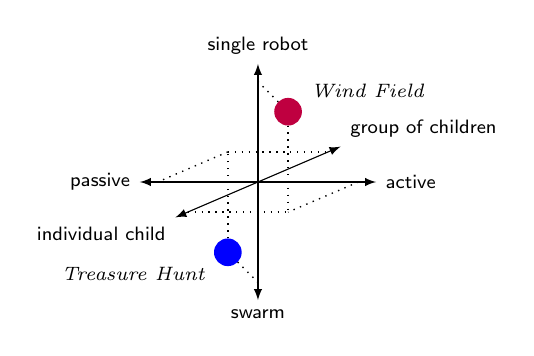
\begin{tikzpicture}[
            >=latex,
            scale=1.5,
            font=\sf\scriptsize,
            spacedots/.style={dotted, black, line width=0.5pt},
            studycircle/.style={circle, inner sep=0pt, minimum size = 1em}
        ]
        \def\xaxis{1};
        \def\zaxis{1};
        \def\yaxisxcoeff{0.7};
        \def\yaxiszcoeff{0.3};
        \def\yaxisx{\yaxisxcoeff*\xaxis};
        \def\yaxisz{\yaxiszcoeff*\zaxis};

        %Axes

        \draw[<->] (-\xaxis,0) -- (\xaxis,0) node[at end,right] {active} node[at start,left] {passive};
        \draw[<->] (0,-\zaxis) -- (0,\zaxis) node[at end,above] {single robot} node[at start,below] {swarm};
        \draw[<->] (-\yaxisx,-\yaxisz) -- (\yaxisx,\yaxisz) node[at end,above,anchor=south west] {group of children} node[at start,below,anchor=north east] {individual child};

        \def\projcoeff{0.85};

        %% Study 1: Treasure hunt

        \def\StudyOneXProjOne{-\projcoeff*\xaxis};  \def\StudyOneXProjTwo{0};
        \def\StudyOneYProjOne{\projcoeff*\yaxisx};  \def\StudyOneYProjTwo{\projcoeff*\yaxisz};
        \def\StudyOneZProjOne{0};                   \def\StudyOneZProjTwo{-\projcoeff*\zaxis};

        \coordinate (study1_xproj) at (\StudyOneXProjOne,\StudyOneXProjTwo);
        \coordinate (study1_yproj) at (\StudyOneYProjOne,\StudyOneYProjTwo);
        \coordinate (study1_zproj) at (\StudyOneZProjOne,\StudyOneZProjTwo);
        \coordinate (study1_xyproj) at (\StudyOneYProjOne + \StudyOneXProjOne, \StudyOneYProjTwo);
        \coordinate (study1) at (\StudyOneYProjOne + \StudyOneXProjOne, \StudyOneYProjTwo + \StudyOneZProjTwo);

        \draw[spacedots] (study1) -- (study1_xyproj);
        \draw[spacedots] (study1_xyproj) -- (study1_xproj);
        \draw[spacedots] (study1_xyproj) -- (study1_yproj);
        \draw[spacedots] (study1) -- (study1_zproj);
        \node[studycircle,fill=blue] at (study1) [label=200:\it Treasure Hunt] {};

        %% Study 2: Windfield

        \def\StudyTwoXProjOne{\projcoeff*\xaxis};   \def\StudyTwoXProjTwo{0};
        \def\StudyTwoYProjOne{-\projcoeff*\yaxisx}; \def\StudyTwoYProjTwo{-\projcoeff*\yaxisz};
        \def\StudyTwoZProjOne{0};                   \def\StudyTwoZProjTwo{\projcoeff*\zaxis};

        \coordinate (study2_xproj) at (\StudyTwoXProjOne, \StudyTwoXProjTwo);
        \coordinate (study2_yproj) at (\StudyTwoYProjOne, \StudyTwoYProjTwo);
        \coordinate (study2_zproj) at (\StudyTwoZProjOne, \StudyTwoZProjTwo);
        \coordinate (study2_xyproj) at (\StudyTwoYProjOne + \StudyTwoXProjOne, \StudyTwoYProjTwo);
        \coordinate (study2) at (\StudyTwoYProjOne + \StudyTwoXProjOne, \StudyTwoYProjTwo + \StudyTwoZProjTwo);

        \draw[spacedots] (study2) -- (study2_xyproj);
        \draw[spacedots] (study2_yproj) -- (study2_xyproj);
        \draw[spacedots] (study2_xproj) -- (study2_xyproj);
        \draw[spacedots] (study2) -- (study2_zproj);
        \node[studycircle,fill=purple] at (study2) [label=20:\it Wind Field] {};

    \end{tikzpicture}
    \caption{}

    \label{fig:adapation-space}
\end{figure}